\documentclass[11pt,a4paper,]{article}
\usepackage{lmodern}

\usepackage{amssymb,amsmath}
\usepackage{ifxetex,ifluatex}
\usepackage{fixltx2e} % provides \textsubscript
\ifnum 0\ifxetex 1\fi\ifluatex 1\fi=0 % if pdftex
  \usepackage[T1]{fontenc}
  \usepackage[utf8]{inputenc}
\else % if luatex or xelatex
  \usepackage{unicode-math}
  \defaultfontfeatures{Ligatures=TeX,Scale=MatchLowercase}
\fi
% use upquote if available, for straight quotes in verbatim environments
\IfFileExists{upquote.sty}{\usepackage{upquote}}{}
% use microtype if available
\IfFileExists{microtype.sty}{%
\usepackage[]{microtype}
\UseMicrotypeSet[protrusion]{basicmath} % disable protrusion for tt fonts
}{}
\PassOptionsToPackage{hyphens}{url} % url is loaded by hyperref
\usepackage[unicode=true]{hyperref}
\hypersetup{
            pdftitle={ETC5513\_Assignment4},
            pdfborder={0 0 0},
            breaklinks=true}
\urlstyle{same}  % don't use monospace font for urls
\usepackage{geometry}
\geometry{a4paper, centering, text={16cm,24cm}}
\usepackage[style=authoryear-comp,]{biblatex}
\addbibresource{references.bib}
\usepackage{color}
\usepackage{fancyvrb}
\newcommand{\VerbBar}{|}
\newcommand{\VERB}{\Verb[commandchars=\\\{\}]}
\DefineVerbatimEnvironment{Highlighting}{Verbatim}{commandchars=\\\{\}}
% Add ',fontsize=\small' for more characters per line
\usepackage{framed}
\definecolor{shadecolor}{RGB}{248,248,248}
\newenvironment{Shaded}{\begin{snugshade}}{\end{snugshade}}
\newcommand{\AlertTok}[1]{\textcolor[rgb]{0.94,0.16,0.16}{#1}}
\newcommand{\AnnotationTok}[1]{\textcolor[rgb]{0.56,0.35,0.01}{\textbf{\textit{#1}}}}
\newcommand{\AttributeTok}[1]{\textcolor[rgb]{0.77,0.63,0.00}{#1}}
\newcommand{\BaseNTok}[1]{\textcolor[rgb]{0.00,0.00,0.81}{#1}}
\newcommand{\BuiltInTok}[1]{#1}
\newcommand{\CharTok}[1]{\textcolor[rgb]{0.31,0.60,0.02}{#1}}
\newcommand{\CommentTok}[1]{\textcolor[rgb]{0.56,0.35,0.01}{\textit{#1}}}
\newcommand{\CommentVarTok}[1]{\textcolor[rgb]{0.56,0.35,0.01}{\textbf{\textit{#1}}}}
\newcommand{\ConstantTok}[1]{\textcolor[rgb]{0.00,0.00,0.00}{#1}}
\newcommand{\ControlFlowTok}[1]{\textcolor[rgb]{0.13,0.29,0.53}{\textbf{#1}}}
\newcommand{\DataTypeTok}[1]{\textcolor[rgb]{0.13,0.29,0.53}{#1}}
\newcommand{\DecValTok}[1]{\textcolor[rgb]{0.00,0.00,0.81}{#1}}
\newcommand{\DocumentationTok}[1]{\textcolor[rgb]{0.56,0.35,0.01}{\textbf{\textit{#1}}}}
\newcommand{\ErrorTok}[1]{\textcolor[rgb]{0.64,0.00,0.00}{\textbf{#1}}}
\newcommand{\ExtensionTok}[1]{#1}
\newcommand{\FloatTok}[1]{\textcolor[rgb]{0.00,0.00,0.81}{#1}}
\newcommand{\FunctionTok}[1]{\textcolor[rgb]{0.00,0.00,0.00}{#1}}
\newcommand{\ImportTok}[1]{#1}
\newcommand{\InformationTok}[1]{\textcolor[rgb]{0.56,0.35,0.01}{\textbf{\textit{#1}}}}
\newcommand{\KeywordTok}[1]{\textcolor[rgb]{0.13,0.29,0.53}{\textbf{#1}}}
\newcommand{\NormalTok}[1]{#1}
\newcommand{\OperatorTok}[1]{\textcolor[rgb]{0.81,0.36,0.00}{\textbf{#1}}}
\newcommand{\OtherTok}[1]{\textcolor[rgb]{0.56,0.35,0.01}{#1}}
\newcommand{\PreprocessorTok}[1]{\textcolor[rgb]{0.56,0.35,0.01}{\textit{#1}}}
\newcommand{\RegionMarkerTok}[1]{#1}
\newcommand{\SpecialCharTok}[1]{\textcolor[rgb]{0.00,0.00,0.00}{#1}}
\newcommand{\SpecialStringTok}[1]{\textcolor[rgb]{0.31,0.60,0.02}{#1}}
\newcommand{\StringTok}[1]{\textcolor[rgb]{0.31,0.60,0.02}{#1}}
\newcommand{\VariableTok}[1]{\textcolor[rgb]{0.00,0.00,0.00}{#1}}
\newcommand{\VerbatimStringTok}[1]{\textcolor[rgb]{0.31,0.60,0.02}{#1}}
\newcommand{\WarningTok}[1]{\textcolor[rgb]{0.56,0.35,0.01}{\textbf{\textit{#1}}}}
\usepackage{longtable,booktabs}
% Fix footnotes in tables (requires footnote package)
\IfFileExists{footnote.sty}{\usepackage{footnote}\makesavenoteenv{long table}}{}
\IfFileExists{parskip.sty}{%
\usepackage{parskip}
}{% else
\setlength{\parindent}{0pt}
\setlength{\parskip}{6pt plus 2pt minus 1pt}
}
\setlength{\emergencystretch}{3em}  % prevent overfull lines
\providecommand{\tightlist}{%
  \setlength{\itemsep}{0pt}\setlength{\parskip}{0pt}}
\setcounter{secnumdepth}{5}

% set default figure placement to htbp
\makeatletter
\def\fps@figure{htbp}
\makeatother


\title{ETC5513\_Assignment4}

%% MONASH STUFF

%% CAPTIONS
\RequirePackage{caption}
\DeclareCaptionStyle{italic}[justification=centering]
 {labelfont={bf},textfont={it},labelsep=colon}
\captionsetup[figure]{style=italic,format=hang,singlelinecheck=true}
\captionsetup[table]{style=italic,format=hang,singlelinecheck=true}


%% FONT
\RequirePackage{bera}
\RequirePackage[charter,expert,sfscaled]{mathdesign}
\RequirePackage{fontawesome}

%% HEADERS AND FOOTERS
\RequirePackage{fancyhdr}
\pagestyle{fancy}
\rfoot{\Large\sffamily\raisebox{-0.1cm}{\textbf{\thepage}}}
\makeatletter
\lhead{\textsf{\expandafter{\@title}}}
\makeatother
\rhead{}
\cfoot{}
\setlength{\headheight}{15pt}
\renewcommand{\headrulewidth}{0.4pt}
\renewcommand{\footrulewidth}{0.4pt}
\fancypagestyle{plain}{%
\fancyhf{} % clear all header and footer fields
\fancyfoot[C]{\sffamily\thepage} % except the center
\renewcommand{\headrulewidth}{0pt}
\renewcommand{\footrulewidth}{0pt}}

%% MATHS
\RequirePackage{bm,amsmath}
\allowdisplaybreaks

%% GRAPHICS
\RequirePackage{graphicx}
\setcounter{topnumber}{2}
\setcounter{bottomnumber}{2}
\setcounter{totalnumber}{4}
\renewcommand{\topfraction}{0.85}
\renewcommand{\bottomfraction}{0.85}
\renewcommand{\textfraction}{0.15}
\renewcommand{\floatpagefraction}{0.8}


%\RequirePackage[section]{placeins}

%% SECTION TITLES


%% SECTION TITLES (NEW: Changing sections and subsections color)
\RequirePackage[compact,sf,bf]{titlesec}
\titleformat*{\section}{\Large\sf\bfseries\color[rgb]{0.8, 0.7, 0.1 }}
\titleformat*{\subsection}{\large\sf\bfseries\color[rgb]{0.8, 0.7, 0.1 }}
\titleformat*{\subsubsection}{\sf\bfseries\color[rgb]{0.8, 0.7, 0.1 }}
\titlespacing{\section}{0pt}{2ex}{.5ex}
\titlespacing{\subsection}{0pt}{1.5ex}{0ex}
\titlespacing{\subsubsection}{0pt}{.5ex}{0ex}


%% TITLE PAGE
\def\Date{\number\day}
\def\Month{\ifcase\month\or
 January\or February\or March\or April\or May\or June\or
 July\or August\or September\or October\or November\or December\fi}
\def\Year{\number\year}

%% LINE AND PAGE BREAKING
\sloppy
\clubpenalty = 10000
\widowpenalty = 10000
\brokenpenalty = 10000
\RequirePackage{microtype}

%% PARAGRAPH BREAKS
\setlength{\parskip}{1.4ex}
\setlength{\parindent}{0em}

%% HYPERLINKS
\RequirePackage{xcolor} % Needed for links
\definecolor{darkblue}{rgb}{0,0,.6}
\RequirePackage{url}

\makeatletter
\@ifpackageloaded{hyperref}{}{\RequirePackage{hyperref}}
\makeatother
\hypersetup{
     citecolor=0 0 0,
     breaklinks=true,
     bookmarksopen=true,
     bookmarksnumbered=true,
     linkcolor=darkblue,
     urlcolor=blue,
     citecolor=darkblue,
     colorlinks=true}

\usepackage[showonlyrefs]{mathtools}
\usepackage[no-weekday]{eukdate}

%% BIBLIOGRAPHY

\makeatletter
\@ifpackageloaded{biblatex}{}{\usepackage[style=authoryear-comp, backend=biber, natbib=true]{biblatex}}
\makeatother
\ExecuteBibliographyOptions{bibencoding=utf8,minnames=1,maxnames=3, maxbibnames=99,dashed=false,terseinits=true,giveninits=true,uniquename=false,uniquelist=false,doi=false, isbn=false,url=true,sortcites=false}

\DeclareFieldFormat{url}{\texttt{\url{#1}}}
\DeclareFieldFormat[article]{pages}{#1}
\DeclareFieldFormat[inproceedings]{pages}{\lowercase{pp.}#1}
\DeclareFieldFormat[incollection]{pages}{\lowercase{pp.}#1}
\DeclareFieldFormat[article]{volume}{\mkbibbold{#1}}
\DeclareFieldFormat[article]{number}{\mkbibparens{#1}}
\DeclareFieldFormat[article]{title}{\MakeCapital{#1}}
\DeclareFieldFormat[article]{url}{}
%\DeclareFieldFormat[book]{url}{}
%\DeclareFieldFormat[inbook]{url}{}
%\DeclareFieldFormat[incollection]{url}{}
%\DeclareFieldFormat[inproceedings]{url}{}
\DeclareFieldFormat[inproceedings]{title}{#1}
\DeclareFieldFormat{shorthandwidth}{#1}
%\DeclareFieldFormat{extrayear}{}
% No dot before number of articles
\usepackage{xpatch}
\xpatchbibmacro{volume+number+eid}{\setunit*{\adddot}}{}{}{}
% Remove In: for an article.
\renewbibmacro{in:}{%
  \ifentrytype{article}{}{%
  \printtext{\bibstring{in}\intitlepunct}}}

\AtEveryBibitem{\clearfield{month}}
\AtEveryCitekey{\clearfield{month}}

\makeatletter
\DeclareDelimFormat[cbx@textcite]{nameyeardelim}{\addspace}
\makeatother

\author{\sf\Large\textbf{ Peizhao Chen}\\ {\sf\large XXX\\[0.5cm]} \sf\Large\textbf{ Xinyi Tang}\\ {\sf\large XXX\\[0.5cm]} \sf\Large\textbf{ XXX XXX}\\ {\sf\large XXX\\[0.5cm]}}

\date{\sf\Date~\Month~\Year}
\makeatletter
\lfoot{\sf Chen, Tang, XXX: \@date}
\makeatother


%%%% PAGE STYLE FOR FRONT PAGE OF REPORTS

\makeatletter
\def\organization#1{\gdef\@organization{#1}}
\def\telephone#1{\gdef\@telephone{#1}}
\def\email#1{\gdef\@email{#1}}
\makeatother
  \organization{Australian Government COVID19}

  \def\name{Our consultancy \newline add names \&\newline add names}

  \telephone{(03) 9905 2478}

  \email{questions@company.com}                 %NEW: New email addresss

\def\webaddress{\url{http://company.com/stats/consulting/}} %NEW: URl
\def\abn{12 377 614 630}                                    % NEW: ABN
\def\logo{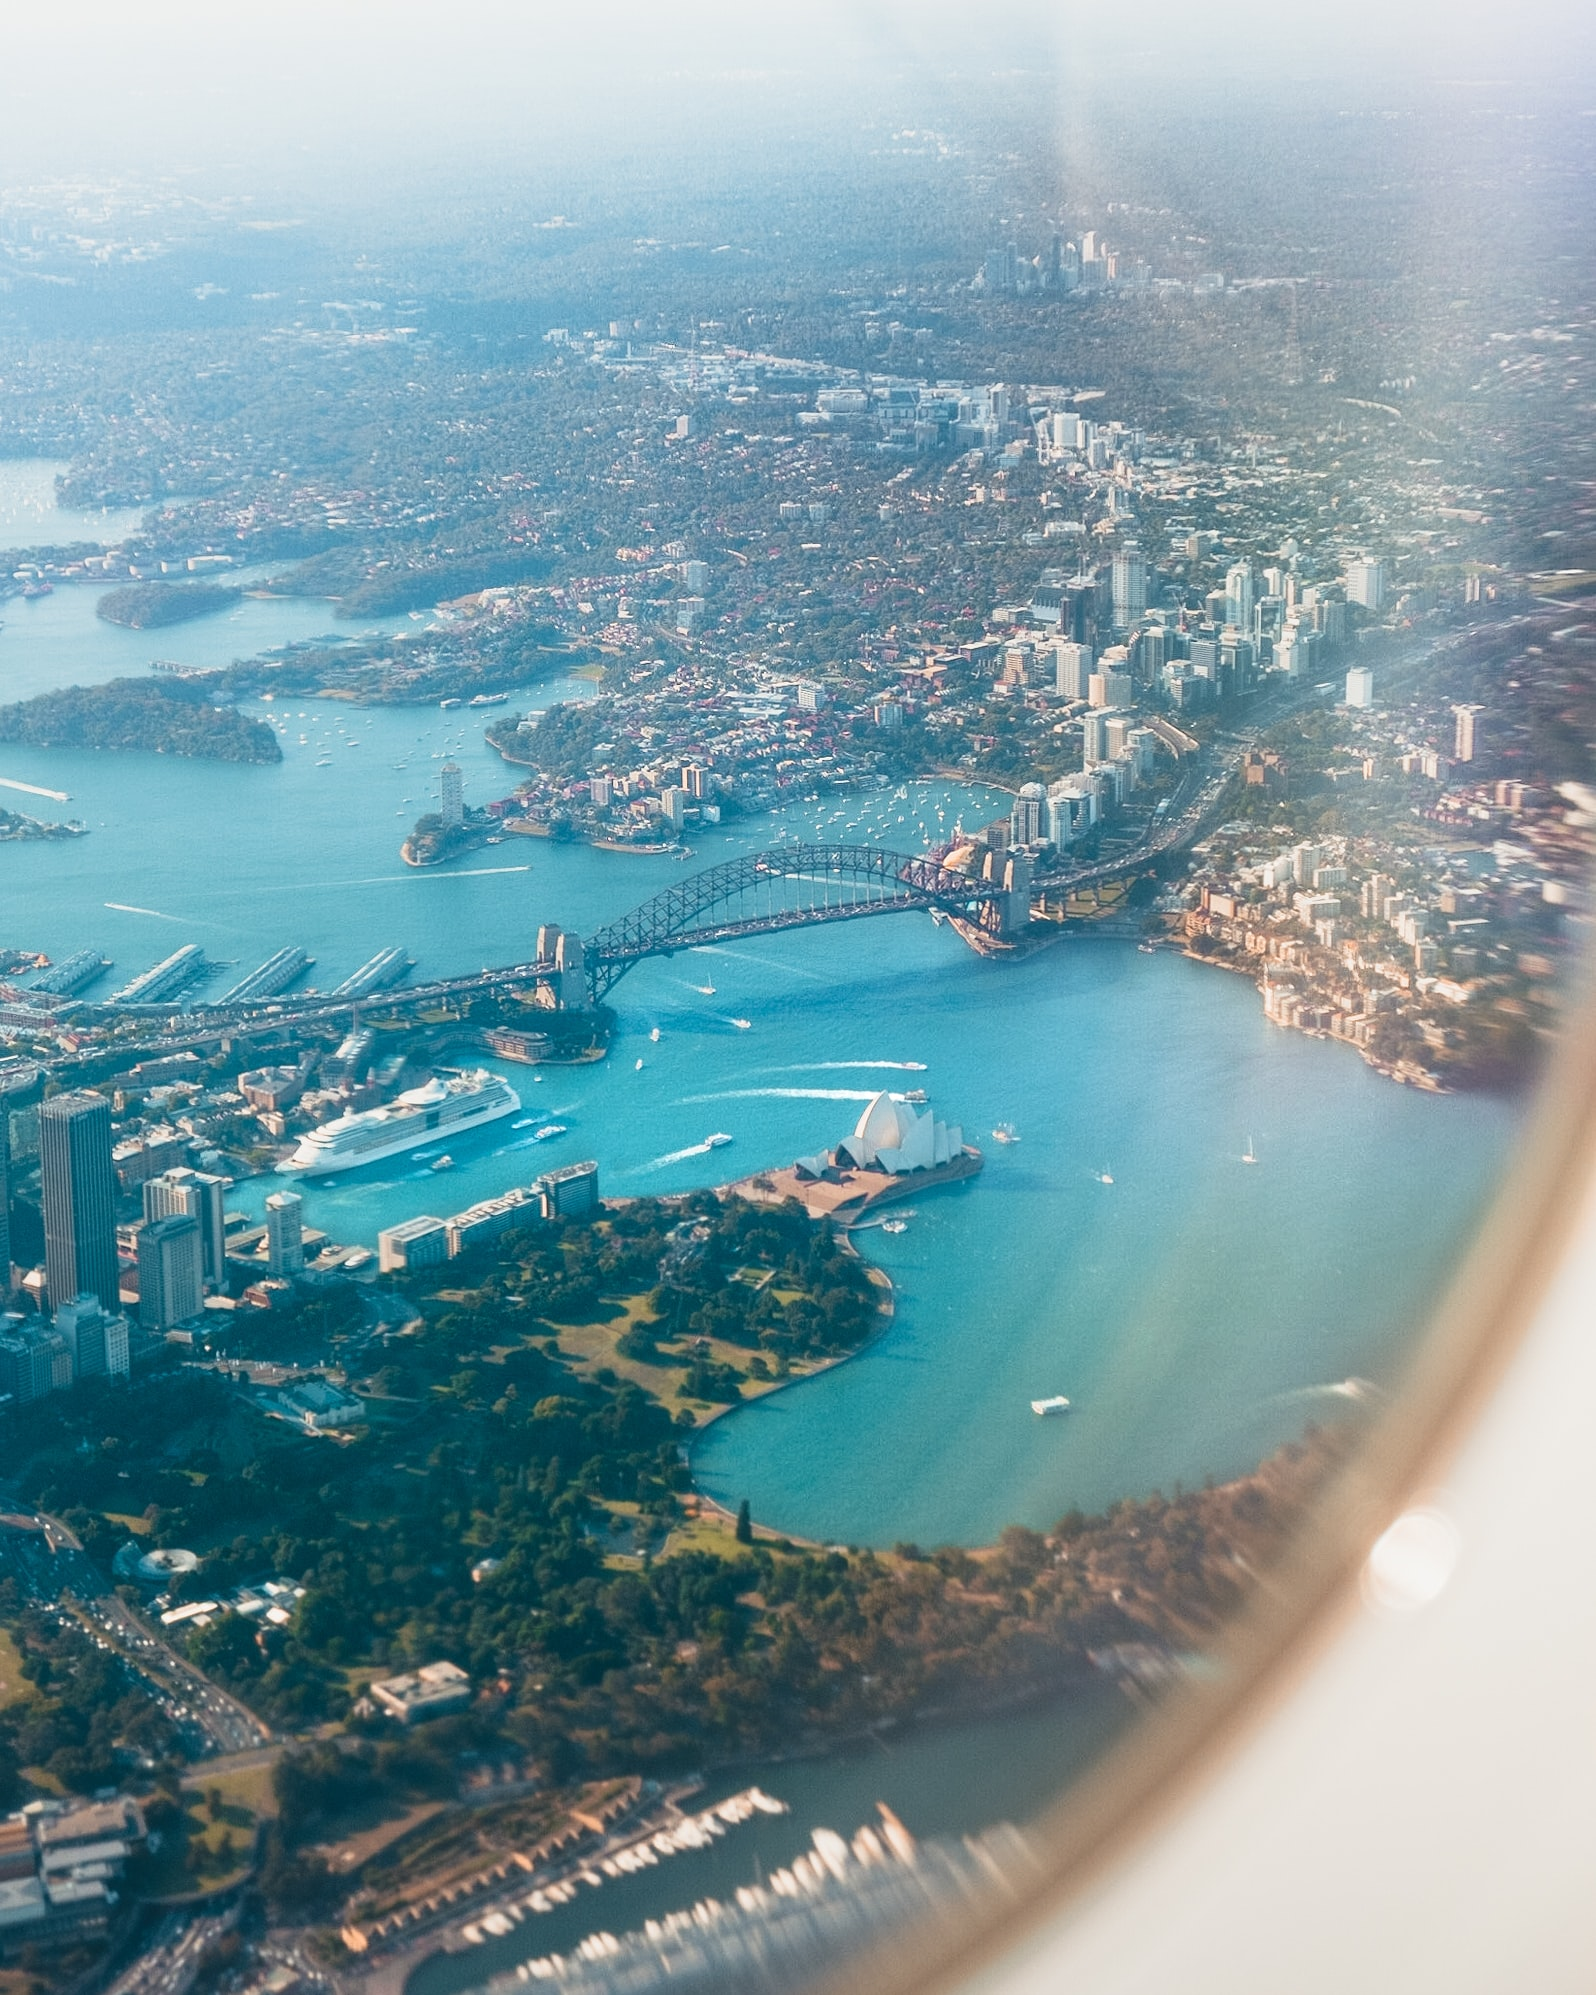
\includegraphics[width=6cm]{logo}}  %NEW: Changing logo
\def\extraspace{\vspace*{1.6cm}}
\makeatletter
\def\contactdetails{\faicon{phone} & \@telephone \\
                    \faicon{envelope} & \@email}
\makeatother

%%%% FRONT PAGE OF REPORTS

\def\reporttype{Report for}

\long\def\front#1#2#3{
\newpage
\begin{singlespacing}
\thispagestyle{empty}
\vspace*{-1.4cm}
\hspace*{-1.4cm}
\hbox to 16cm{
  \hbox to 6.5cm{\vbox to 14cm{\vbox to 25cm{
    \logo
    \vfill
    \parbox{6.3cm}{\raggedright
      \sf\color[rgb]{0.8, 0.7, 0.1 }    % NEW color 
      {\large\textbf{\name}}\par
      \vspace{.7cm}
      \tabcolsep=0.12cm\sf\small
      \begin{tabular}{@{}ll@{}}\contactdetails
      \end{tabular}
      \vspace*{0.3cm}\par
      ABN: \abn\par
    }
  }\vss}\hss}
  \hspace*{0.2cm}
  \hbox to 1cm{\vbox to 14cm{\rule{4pt}{26.8cm}\vss}\hss\hfill}  %NEW: Thicker line
  \hbox to 10cm{\vbox to 14cm{\vbox to 25cm{   
      \vspace*{3cm}\sf\raggedright
      \parbox{11cm}{\sf\raggedright\baselineskip=1.2cm
         \fontsize{24.88}{30}\color[rgb]{0, 0.29, 0.55}\sf\textbf{#1}}   % NEW: title color blue
      \par
      \vfill
      \large
      \vbox{\parskip=0.8cm #2}\par
      \vspace*{2cm}\par
      \reporttype\\[0.3cm]
      \hbox{#3}%\\[2cm]\
      \vspace*{1cm}
      {\large\sf\textbf{\Date~\Month~\Year}}
   }\vss}
  }}
\end{singlespacing}
\newpage
}

\makeatletter
\def\titlepage{\front{\expandafter{\@title}}{\@author}{\@organization}}
\makeatother

\usepackage{setspace}
\setstretch{1.5}

%% Any special functions or other packages can be loaded here.
\usepackage{booktabs}
\usepackage{longtable}
\usepackage{array}
\usepackage{multirow}
\usepackage{wrapfig}
\usepackage{float}
\usepackage{colortbl}
\usepackage{pdflscape}
\usepackage{tabu}
\usepackage{threeparttable}
\usepackage{threeparttablex}
\usepackage[normalem]{ulem}
\usepackage{makecell}
\usepackage{xcolor}


\begin{document}
\titlepage

\section*{Overall analysis from 1990 to 2013}

\hypertarget{introduction}{%
\section{Introduction}\label{introduction}}

This report aims to analyze factors related to GDP growth from 1990 to 2019 in Australia.There are several parts we want to figure out by analyzing the data: overall changes in unemployment,population,GDP growth,unemployment with different education level,and unemployment by genders from 1990 to 2020.The comparison between different categories of unemployment.The factors related to the GDP growth and their relations.
The report is based on the Data of the world bank.All data of ABS presented on this website is provided under a Creative Commons Attribution 4.0 International license, it is open data and free to share and adapt for any purpose even commercially.

\begin{table}[H]

\caption{\label{tab:m1}Missing values in data}
\centering
\begin{tabular}[t]{lrr}
\toprule
variable & n\_miss & pct\_miss\\
\midrule
Advanced\_edu & 7 & 29.16667\\
Basic\_edu & 7 & 29.16667\\
year & 0 & 0.00000\\
GDP\_growth & 0 & 0.00000\\
Population & 0 & 0.00000\\
\addlinespace
Unemploy\_F & 0 & 0.00000\\
Unemploy\_M & 0 & 0.00000\\
Inflation & 0 & 0.00000\\
Unemploy\_T & 0 & 0.00000\\
\bottomrule
\end{tabular}
\end{table}

From the given table \ref{tab:m1}There are significant proportion of missing values in variables unemployment with advanced education and basic education.That means the research concerning these two variables should begin at 2000 .

\begin{Shaded}
\begin{Highlighting}[]
\NormalTok{g1 }\OtherTok{\textless{}{-}}\NormalTok{ AUS }\SpecialCharTok{\%\textgreater{}\%} 
  \FunctionTok{ggplot}\NormalTok{(}\FunctionTok{aes}\NormalTok{(year,gdp\_growth)) }\SpecialCharTok{+}
  \FunctionTok{geom\_line}\NormalTok{()}\SpecialCharTok{+}
  \FunctionTok{labs}\NormalTok{(}\AttributeTok{x =} \StringTok{"Year"}\NormalTok{,}
       \AttributeTok{y =} \StringTok{"percentage of GDP change"}\NormalTok{)}
\end{Highlighting}
\end{Shaded}

From the given figure \ref{fig:g1},only the beginning of 1990s has experienced a negative growth which was about -0.3\%,and the following growth of years was fluctuating around 2.5\% even after 2008 the year of financial crisis the growth is still positive.The negative growth in 1990s attribute to recession mainly resulted from Australia's efforts to address excess domestic demand,.curb speculative behaviour in commercial property markets and reduce inflation. Interest rates were increased to a very high level because the transmission of tighter monetary policy took longer than expected to put downward pressure on demand and inflation.

\begin{Shaded}
\begin{Highlighting}[]
\NormalTok{g2 }\OtherTok{\textless{}{-}}\NormalTok{ AUS }\SpecialCharTok{\%\textgreater{}\%} 
  \FunctionTok{ggplot}\NormalTok{(}\FunctionTok{aes}\NormalTok{(year,population)) }\SpecialCharTok{+}
  \FunctionTok{geom\_line}\NormalTok{()}\SpecialCharTok{+}
  \FunctionTok{scale\_y\_continuous}\NormalTok{(}\AttributeTok{labels =}\NormalTok{ scales}\SpecialCharTok{::}\NormalTok{comma) }\SpecialCharTok{+}
  \FunctionTok{labs}\NormalTok{(}\AttributeTok{x =} \StringTok{"Year"}\NormalTok{,}
       \AttributeTok{y =} \StringTok{"Population"}\NormalTok{)}
\end{Highlighting}
\end{Shaded}

From the given figure \ref{fig:g2}, the Australian population has been growing steadily from 17,000,000 to over 25,000,000 in the year between 1990 to 2020.Australia has population growth rate around 1.48\% averagely according to worldbank data.Migration and birth rate minus mortality rate were included in this growth rate.

\begin{Shaded}
\begin{Highlighting}[]
\NormalTok{g3 }\OtherTok{\textless{}{-}}\NormalTok{ AUS1 }\SpecialCharTok{\%\textgreater{}\%}
  \FunctionTok{ggplot}\NormalTok{(}\FunctionTok{aes}\NormalTok{(year,  }\StringTok{\textasciigrave{}}\AttributeTok{Inflation, consumer prices (annual \%)}\StringTok{\textasciigrave{}}\NormalTok{)) }\SpecialCharTok{+}
  \FunctionTok{geom\_line}\NormalTok{() }\SpecialCharTok{+}
  \FunctionTok{labs}\NormalTok{(}\AttributeTok{x =} \StringTok{"Year"}\NormalTok{,}
       \AttributeTok{y =} \StringTok{"Inflation rate"}\NormalTok{)}
\end{Highlighting}
\end{Shaded}

From the given figure \ref{fig:g3},The inflation rate was fluctuating throughout two decades.The pinnacle was in 1990,about 7\% that is main attribute to the recession,While lowest point was given at 1994.

\begin{table}[H]

\caption{\label{tab:educhange}Percent change in umemployment with different education level}
\centering
\begin{tabular}[t]{r|r|r|l|l}
\hline
year & unemploy\_adv\_edu & unemploy\_bas\_edu & unemploy\_adv\_edu\_change & unemploy\_bas\_edu\_change\\
\hline
2000 & 3.65 & 10.250000 & NA & NA\\
\hline
2001 & 3.36 & 10.650000 & -7.95\% & 3.9\%\\
\hline
2002 & 3.46 & 9.960000 & 2.98\% & -6.48\%\\
\hline
2003 & 3.60 & 9.580000 & 4.05\% & -3.82\%\\
\hline
2004 & 3.25 & 8.680000 & -9.72\% & -9.39\%\\
\hline
2005 & 3.02 & 8.770001 & -7.08\% & 1.04\%\\
\hline
2006 & 2.31 & 7.990000 & -23.51\% & -8.89\%\\
\hline
2007 & 2.37 & 9.240000 & 2.6\% & 15.64\%\\
\hline
2008 & 2.47 & 9.560000 & 4.22\% & 3.46\%\\
\hline
2009 & 3.65 & 9.229999 & 47.77\% & -3.45\%\\
\hline
2010 & 3.02 & 9.070000 & -17.26\% & -1.73\%\\
\hline
2011 & 3.16 & 8.610000 & 4.64\% & -5.07\%\\
\hline
2012 & 3.03 & 9.240000 & -4.11\% & 7.32\%\\
\hline
2013 & 3.42 & 8.630000 & 12.87\% & -6.6\%\\
\hline
\end{tabular}
\end{table}

From the given table \ref{tab:educhange},the unemployment rate of people with advanced education is much lower than people with basic education,which was changing at the rang between 4\% to 2\%.While the unemployment rate for people with basic education is about 10\% to 8\% throughout 13 years.

\begin{center}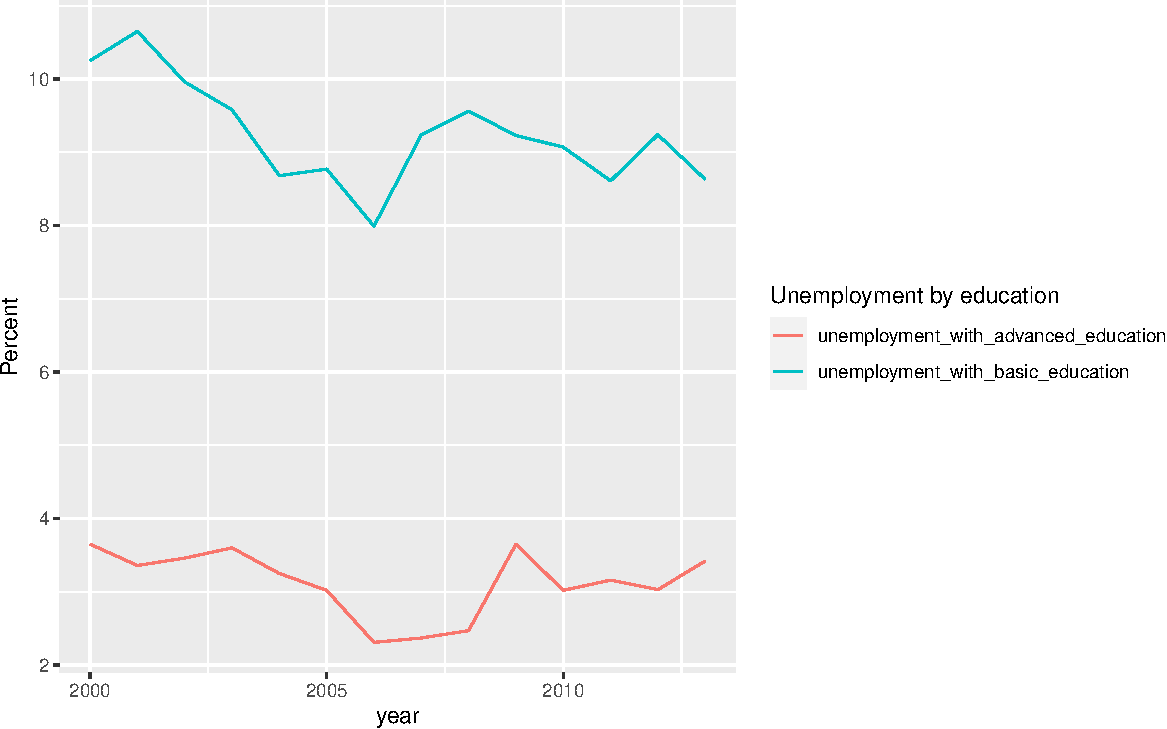
\includegraphics{Figures/g9-1} \end{center}

The given figure \ref{fig:g9} can demonstrate the change more obviously,the two lines are in completely different levels,that means the unemployment of basic education is much more higher than people with advanced education.However,they changes show similar pattern such as the downward trend from 1990 to 2006 and upward from 2007 to 2009.

\begin{table}[H]

\caption{\label{tab:sexchange}Percent change in umemployment by gender}
\centering
\begin{tabular}[t]{r|r|r|l|l}
\hline
year & Unemploy\_F & Unemploy\_M & Unemploy\_F\_Change & Unemploy\_M\_Change\\
\hline
1990 & 7.19 & 6.740000 & NA & NA\\
\hline
1991 & 9.15 & 9.890000 & 27.26\% & 46.74\%\\
\hline
1992 & 9.93 & 11.310000 & 8.52\% & 14.36\%\\
\hline
1993 & 10.00 & 11.510000 & 0.7\% & 1.77\%\\
\hline
1994 & 9.36 & 9.979999 & -6.4\% & -13.29\%\\
\hline
1995 & 8.11 & 8.740000 & -13.35\% & -12.42\%\\
\hline
1996 & 8.24 & 8.710000 & 1.6\% & -0.34\%\\
\hline
1997 & 8.07 & 8.580000 & -2.06\% & -1.49\%\\
\hline
1998 & 7.33 & 7.940000 & -9.17\% & -7.46\%\\
\hline
1999 & 6.66 & 7.040000 & -9.14\% & -11.34\%\\
\hline
2000 & 6.06 & 6.460000 & -9.01\% & -8.24\%\\
\hline
2001 & 6.45 & 6.980000 & 6.44\% & 8.05\%\\
\hline
2002 & 6.16 & 6.530000 & -4.5\% & -6.45\%\\
\hline
2003 & 5.98 & 5.890000 & -2.92\% & -9.8\%\\
\hline
2004 & 5.54 & 5.280000 & -7.36\% & -10.36\%\\
\hline
2005 & 5.22 & 4.880000 & -5.78\% & -7.58\%\\
\hline
2006 & 4.92 & 4.670000 & -5.75\% & -4.3\%\\
\hline
2007 & 4.78 & 4.040000 & -2.85\% & -13.49\%\\
\hline
2008 & 4.57 & 3.960000 & -4.39\% & -1.98\%\\
\hline
2009 & 5.40 & 5.690000 & 18.16\% & 43.69\%\\
\hline
2010 & 5.38 & 5.070000 & -0.37\% & -10.9\%\\
\hline
2011 & 5.30 & 4.890000 & -1.49\% & -3.55\%\\
\hline
2012 & 5.33 & 5.140000 & 0.57\% & 5.11\%\\
\hline
2013 & 5.61 & 5.710000 & 5.25\% & 11.09\%\\
\hline
\end{tabular}
\end{table}

From the given table \ref{tab:sexchange},the ratios of unemployment male and females show no apparent differences,which is around 4\% to 10\%,but in 1992 and 1993 women had experienced a high umemployment rate of over 11\% ,the rate for females was soared from the beginning of 1990s.

\begin{table}[H]

\caption{\label{tab:Tchange}Percent change in total umemployment}
\centering
\begin{tabular}[t]{r|r|l}
\hline
year & Unemploy\_T & Unemploy\_T\_Change\\
\hline
1990 & 6.93 & NA\\
\hline
1991 & 9.58 & 38.24\%\\
\hline
1992 & 10.73 & 12\%\\
\hline
1993 & 10.87 & 1.3\%\\
\hline
1994 & 9.72 & -10.58\%\\
\hline
1995 & 8.47 & -12.86\%\\
\hline
1996 & 8.51 & 0.47\%\\
\hline
1997 & 8.36 & -1.76\%\\
\hline
1998 & 7.68 & -8.13\%\\
\hline
1999 & 6.87 & -10.55\%\\
\hline
2000 & 6.28 & -8.59\%\\
\hline
2001 & 6.74 & 7.32\%\\
\hline
2002 & 6.37 & -5.49\%\\
\hline
2003 & 5.93 & -6.91\%\\
\hline
2004 & 5.39 & -9.11\%\\
\hline
2005 & 5.03 & -6.68\%\\
\hline
2006 & 4.78 & -4.97\%\\
\hline
2007 & 4.38 & -8.37\%\\
\hline
2008 & 4.23 & -3.42\%\\
\hline
2009 & 5.56 & 31.44\%\\
\hline
2010 & 5.21 & -6.29\%\\
\hline
2011 & 5.08 & -2.5\%\\
\hline
2012 & 5.22 & 2.76\%\\
\hline
2013 & 5.66 & 8.43\%\\
\hline
\end{tabular}
\end{table}

From the given table \ref{tab:Tchange},the total unemployment rate of Australia showed a generally downward tendency from 1990 to 2013 since in the beginning of 1990 the rate was about 10\% but after 13 years the unemployment rate has decreased to 5.66\% in 2013.

\section{Exploring Unemployment Rate}

\subsection{Unemployment rate plot}

\begin{figure}[H]

{\centering 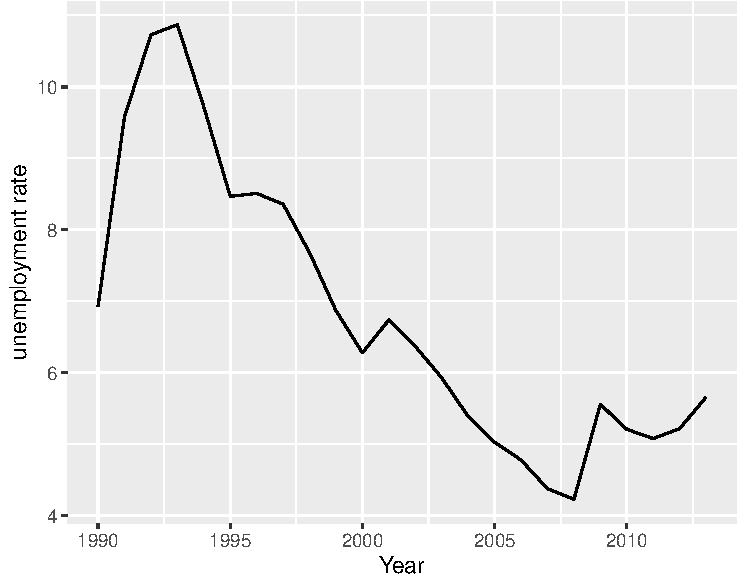
\includegraphics{Figures/unemp-1} 

}

\caption{Unemployment rate from 1990 to 2013}\label{fig:unemp}
\end{figure}

Figure\ref{fig:unemp} shows the changes in the unemployment rate from 19990 to 2013. First, there is a long-run downward trend in the unemployment rate, which is consistent with the idea that Australia's long term unemployment ratio is relatively low amongst other countries in the world. Second, there are two peaks in the graph. The first peak is around the early 1990s, at the time, Australia was experiencing a recession. The second peak is around 2008 due to the global financial crisis.

\subsection{Boxplot}

\begin{figure}[H]

{\centering 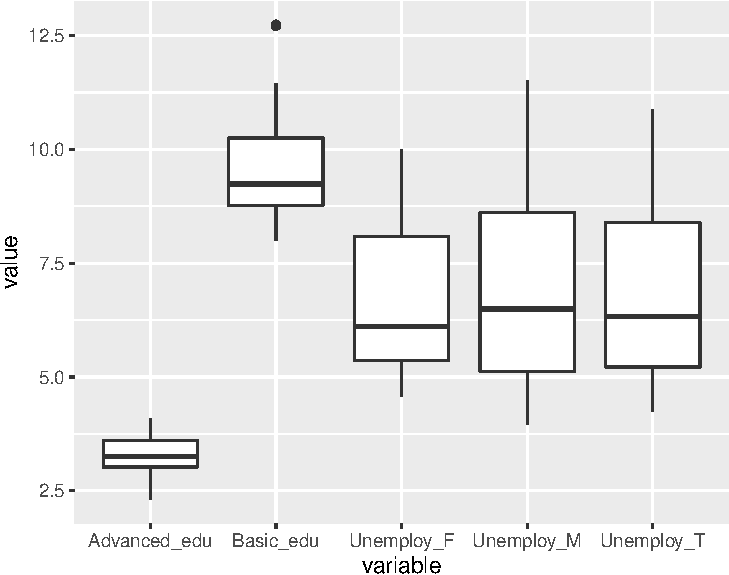
\includegraphics{Figures/boxplot-1} 

}

\caption{Box plot of the unemployment rate}\label{fig:boxplot}
\end{figure}

Figure \ref{fig:boxplot} shows the mean value of advanced education is higher than the mean of the basic education in the boxplot. It means that people with advanced education has a lower unemployment rate than people with basic education.

We also notice that the average male unemployment rate is slightly higher than the female unemployment rate. To see this in details, we are going to plot the unemployment rate by genders.

\subsection{Unemployment rate by genders}

\begin{figure}[H]

{\centering 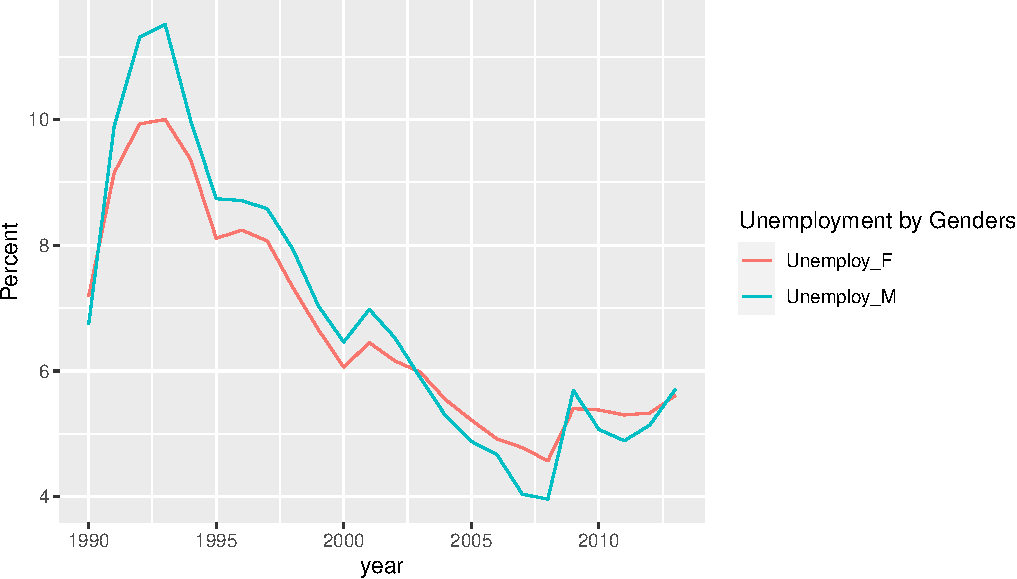
\includegraphics{Figures/gender-1} 

}

\caption{Unemployment rate by genders}\label{fig:gender}
\end{figure}

Figure \ref{fig:gender} shows that female unemployment rates have been consistently below male rates, despite there are some pick-ups in unemployment rates for females over the past few years.

\subsection{Correlation}

\begin{figure}[H]

{\centering 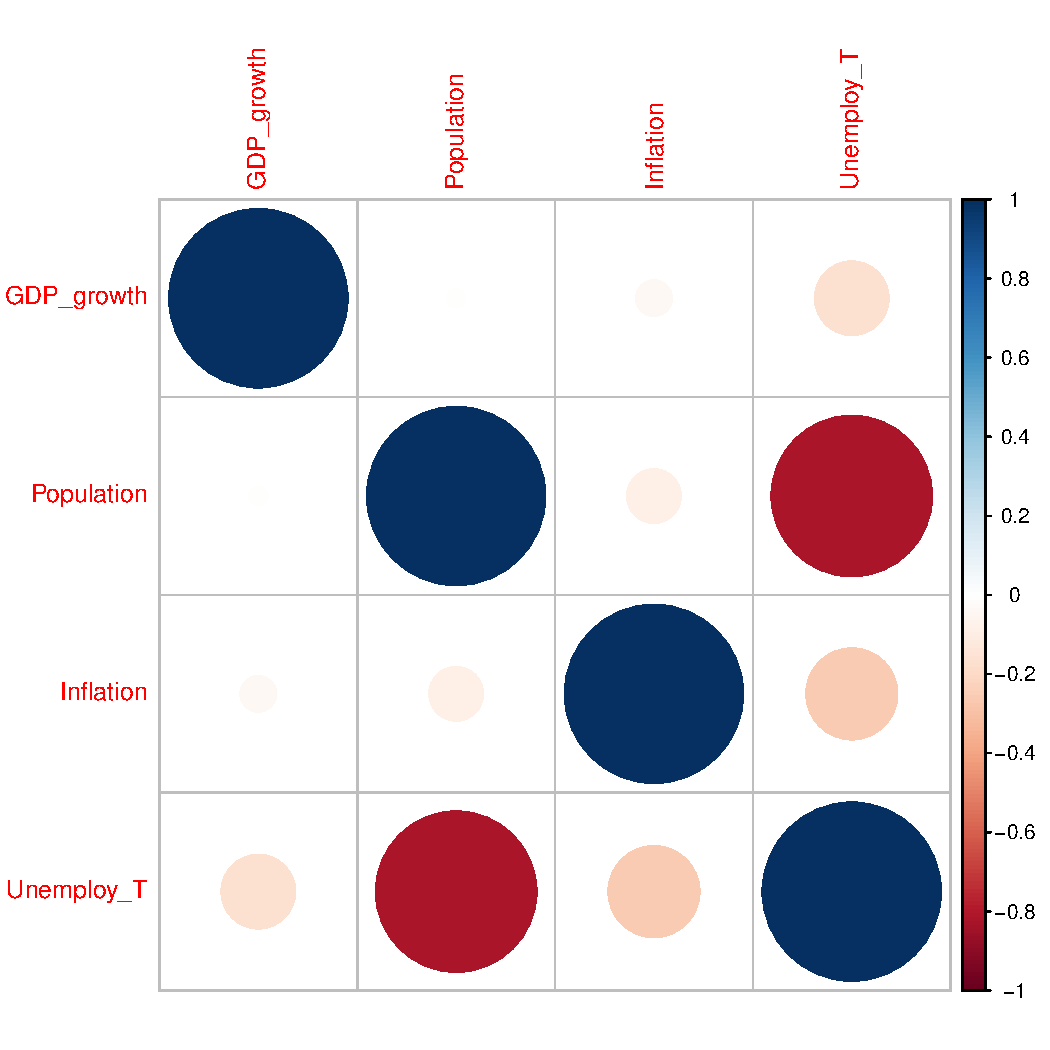
\includegraphics{Figures/cor-1} 

}

\caption{Correlation Graph}\label{fig:cor}
\end{figure}

We expected the unemployment rate has a negative association with GDP. The low unemployment rate would lead to an increase in GDP. Based on the Phillips curve, inflation and the unemployment rate have maintained an inverse relationship historically. Therefore, we expected to see an inverse relationship between inflation and the unemployment rate. Besides, low population growth may lead to a low unemployment rate.

Figure \ref{fig:cor} shows the sign of coefficients as we expected except for the variable population. One possible reason is that the correlation graph could be wrong as it is just an estimation.

\subsection{Linear model for the unemployment rate}

\begin{table}[H]

\caption{\label{tab:model}The estimated linear modelfor the unemployment rate}
\centering
\begin{tabular}[t]{lrrrr}
\toprule
  & Estimate & Std. Error & t value & Pr(>|t|)\\
\midrule
(Intercept) & 27.1939625 & 2.3091897 & 11.776409 & 0.0000000\\
GDP\_growth & -0.3001259 & 0.1556400 & -1.928334 & 0.0681313\\
Population & -0.0000009 & 0.0000001 & -8.371780 & 0.0000001\\
Inflation & -0.4371258 & 0.1294037 & -3.378000 & 0.0029892\\
\bottomrule
\end{tabular}
\end{table}

Based on Figure \ref{fig:cor}, we model the factors that affect the employment rate. Table \ref{tab:model} shows that all the coefficients are significant under the 10\% level of significance. Finally, The value of R squared is equal to 79.95\%. Therefore, the 79.95\% of the variance for the unemployment rate can be explained by GDP\_growth, Population and Inflation.

\section{Country XX3 and YY3}

\textcite{basiceducation}
\textcite{advancededucation}

\printbibliography

\end{document}
